\chapter{\textit{\gls{pop}}}
\label{a:bvm}

\begin{figure}[ht!]
	\begin{center}
		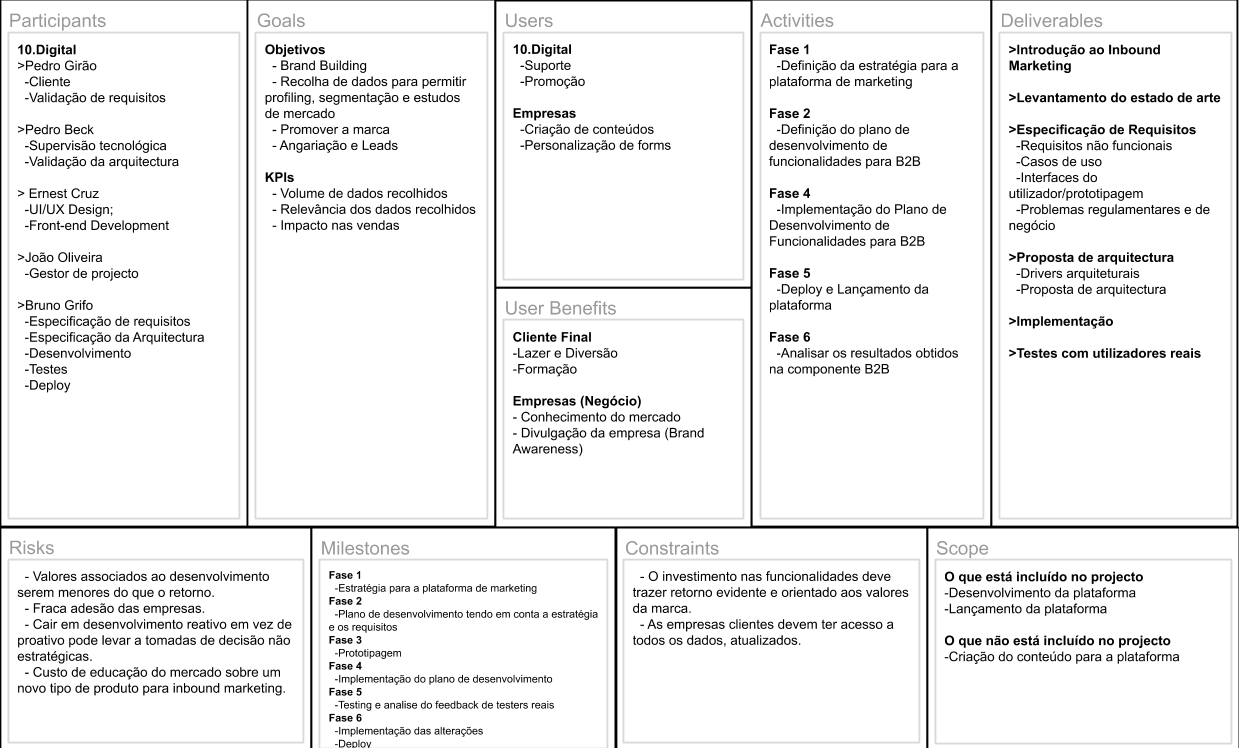
\includegraphics[width=1\textwidth]{img/bmc}
		\caption{10.quest - \textit{\gls{pop}}}
		\label{10q-bmc}
	\end{center}
\end{figure}

Representado na Figura \ref{10q-bmc} temos todo o modelo de negócio da 10.quest representado numa página.

Na secção dos Participantes estão indicados os membros da equipa e os \textit{stakeholders}, os nomes de cada individuo e respectiva função no projecto. 
 
Na secção dos Objectivos é indicado os objetivos principais do projecto, incluindo as métricas de sucesso. 
 
Na Secção dos Utilizadores, estão listados os utilizadores do produto separados por segmentos. 
 
Nos Beneficios dos Utilizadores é representada a proposta de valor e os benefícios que a plataforma traz para os utilizadores. 
 
Na secção das Actividades está a lista concreta de tarefas e acções que a equipa irá ter que realizar para atingir os objetivos do projecto. Nas Entregas estão indicados os resultados e documentos que terão de ser apresentados aos stakeholders ou ao cliente. 
 
Na secção dos Riscos estão identificados possíveis futuros eventos que podem ter um impacto negativo no sucesso do projecto. 
 
Nas Milestones estão listados os pontos críticos que se enquadram na linha temporal do projedcto. 

Na secção das Restrições estão identificados os limites e os requisitos condicionais que afectam diretamente as entregas, actividades ou até mesmo o projecto num todo. 

Por fim temos a secção do Escopo que indica a amplitudo do projeto a ser incluído para consideração, incluindo o que está fora do projeto.